\subsection{OR問題を学習させた際の誤差収束度合いについて}
\subsubsection{実験結果}
NNでは重みを更新する毎に誤差が減るように学習を行うが、
その学習の様子は初期の重みをどのように設定したか、
学習に用いたパラメータをどのように設定したか、
といった対象問題以外の要素に影響して学習の様子が変化する。
シード値を変えた際の学習収束回数を表\ref{table:level1}に示す。
シード値を10回変更して学習させた際の重みを更新する様子を図
\ref{fig:level1-1}に、
その平均をプロットした平均推移値を図\ref{fig:level1-2}に示す。
なお、平均値を求める際には**して**した。
具体的には云々。

\begin{table}[htb]
 \begin{center}
  \caption{OR問題の学習に要した回数}
  \label{table:level1}
  \begin{tabular}[htb]{r|l} \hline
   シード値 & 収束した回数 \\ \hline \hline
   100 & hoge \\ \hline
   200 & hoge \\ \hline
   300 & hoge \\ \hline
   400 & hoge \\ \hline
   500 & hoge \\ \hline
   600 & hoge \\ \hline
   700 & hoge \\ \hline
   800 & hoge \\ \hline
   900 & hoge \\ \hline
   1000 & hoge \\ \hline \hline
   10試行の平均値 & hoge \\ \hline
  \end{tabular}
 \end{center}
\end{table}


\begin{figure}[h]
 \begin{center}
  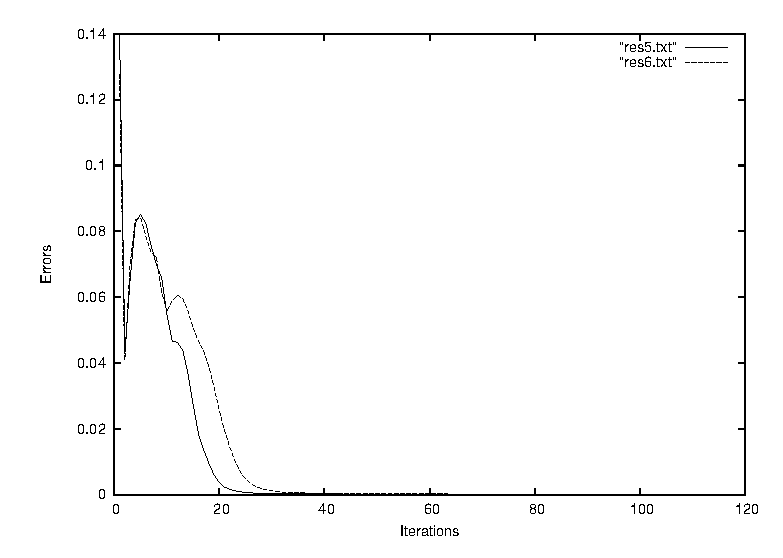
\includegraphics[width=10.0cm]{figs/sample1.eps}
  \caption{重みを更新する様子}
  \label{fig:level1-1}
 \end{center}
\end{figure}

\begin{figure}[h]
 \begin{center}
  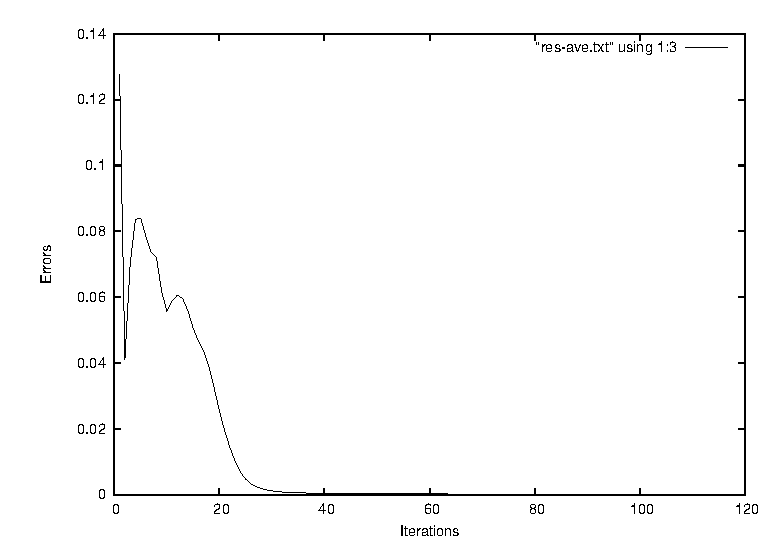
\includegraphics[width=10.0cm]{figs/sample2.eps}
  \caption{重みを更新する様子(平均値)}
  \label{fig:level1-2}
 \end{center}
\end{figure}


\subsubsection{考察}
(結果から分かったことは?)


